\documentclass[12pt]{article}
\usepackage{latexsym}
\usepackage{tikz}
\usetikzlibrary{automata,positioning}


\topmargin = 0.1in \textwidth=5.7in \textheight=8.6in

\oddsidemargin = 0.2in \evensidemargin = 0.2in


\begin{document}

\begin{center}
    Theory of Computation, SPRING 2015 \\
    Homework Problems\\
    Author: Tawheed Abdul-Raheem\\
\end{center}

\smallskip

\begin{enumerate}
    \item L has all strings w such that w does not contain 101
    
 \begin{tikzpicture}[shorten >=1pt,node distance=4cm,on grid,auto] 
   \node[state,initial, accepting] (q_0)   {$q_0$}; 
   \node[state] (q_1) [ right=of q_0] {$q_1$};
   \node[state] (q_2) [ right=of q_1] {$q_2$};
   \node[state] (q_3) [ right=of q_2] {$q_3$};
    \path[->] 
    (q_0) 
       edge  node {1} (q_1)
        edge [loop below] node {0} ()
    (q_1) 
        
        edge  node {0} (q_2)
        edge [loop above] node {1} ()
    (q_2) 
    edge [bend left] node {0} (q_0)
       edge  node {1} (q_3)
        
    (q_3) 
          edge [loop above] node {1} ();          
\end{tikzpicture}

    \item L has all strings w such that w any string of 1's and 0's except 11 and 111
     
 \begin{tikzpicture}[shorten >=1pt,node distance=4cm,on grid,auto] 
   \node[state,initial, accepting] (q_0)   {$q_0$}; 
   \node[state] (q_1) [ right=of q_0] {$q_1$};
   \node[state] (q_2) [ right=of q_1] {$q_2$};
   \node[state] (q_3) [ right=of q_2] {$q_3$};
   \node[state] (q_4) [ below right=of q_1] {$q_4$};
    \path[->] 
    (q_0) 
       edge  node {} (q_1)
       edge  node {0} (q_4)
    (q_1) 
        edge  node {} (q_2)
        edge  node {0} (q_4)
    (q_2)
       edge  node {} (q_3)
       edge  node {} (q_4)
    (q_3) 
          edge  node {1,0} (q_4)
    (q_4)
           edge [loop above] node {0} ()
          edge [loop below] node {1} ();
\end{tikzpicture}
    
    \item L has all strings w such that w contains at least two 0's and at most one 1
 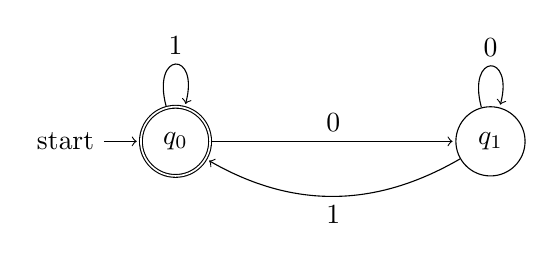
\begin{tikzpicture}[shorten >=1pt,node distance=4cm,on grid,auto] 
   \node[state,initial, accepting] (q_0)   {$q_0$}; 
   \node[state] (q_1) [ right=of q_0] {$q_1$};
    \path[->] 
    (q_0) 
       edge  node {0} (q_1)
        edge [loop above] node {1} ()
        
    (q_1) edge [bend left] node {1} (q_0)
          edge [loop above] node {0} ();
\end{tikzpicture}
\end{enumerate}


\pagebreak

\end{document}
